%!TEX root = ../report.tex
%%%%%%%%%%%%%%%%%%%%%%%%%%%%%%%%%%%%%%%%%%%%%%%%%%%%%%%%%%%%%%%%%%%%%%%
%%%%%%%%%%%%%%%%%%%%%%%%%%%%%%%%%%%%%%%%%%%%%%%%%%%%%%%%%%%%%%%%%%%%%%%
%%%%%                                                                 %
%%%%%     architecture.tex                                            %
%%%%%                                                                 %
%%%%% Author:      Florian Zaruba                                     %
%%%%% Created:     <date>                                             %
%%%%% Description: <description>                                      %
%%%%%                                                                 %
%%%%%%%%%%%%%%%%%%%%%%%%%%%%%%%%%%%%%%%%%%%%%%%%%%%%%%%%%%%%%%%%%%%%%%%
%%%%%%%%%%%%%%%%%%%%%%%%%%%%%%%%%%%%%%%%%%%%%%%%%%%%%%%%%%%%%%%%%%%%%%%

\chapter{Hardware Architecture}

In this chapter I will give an architectural overview of the \pulpino SoC. As described in the instructional chapter both cores available for \pulpino feature a 32-bit 4-stage in order pipeline with distinct ports to the instruction and data RAMs. Since the cores are totally pin compatible one can swap them as needed without modifying any RTL.

\pulpino uses a 32-bit wide AXI as its main interconnect. The memories and the core itself are connected to the AXI Bus via dedicated bus adapters. The APB peripherals are connected to the AXI bus through a AXI2APB adapter. As all components withing the system have access to the AXI bus they share a common memory map. This makes it particularly easy to write and read registers from each peripheral, the core and memories' content. The overall device architecture is depicted in figure~\ref{fig:block_diagram}.


\begin{figure}[th]
  \centering
  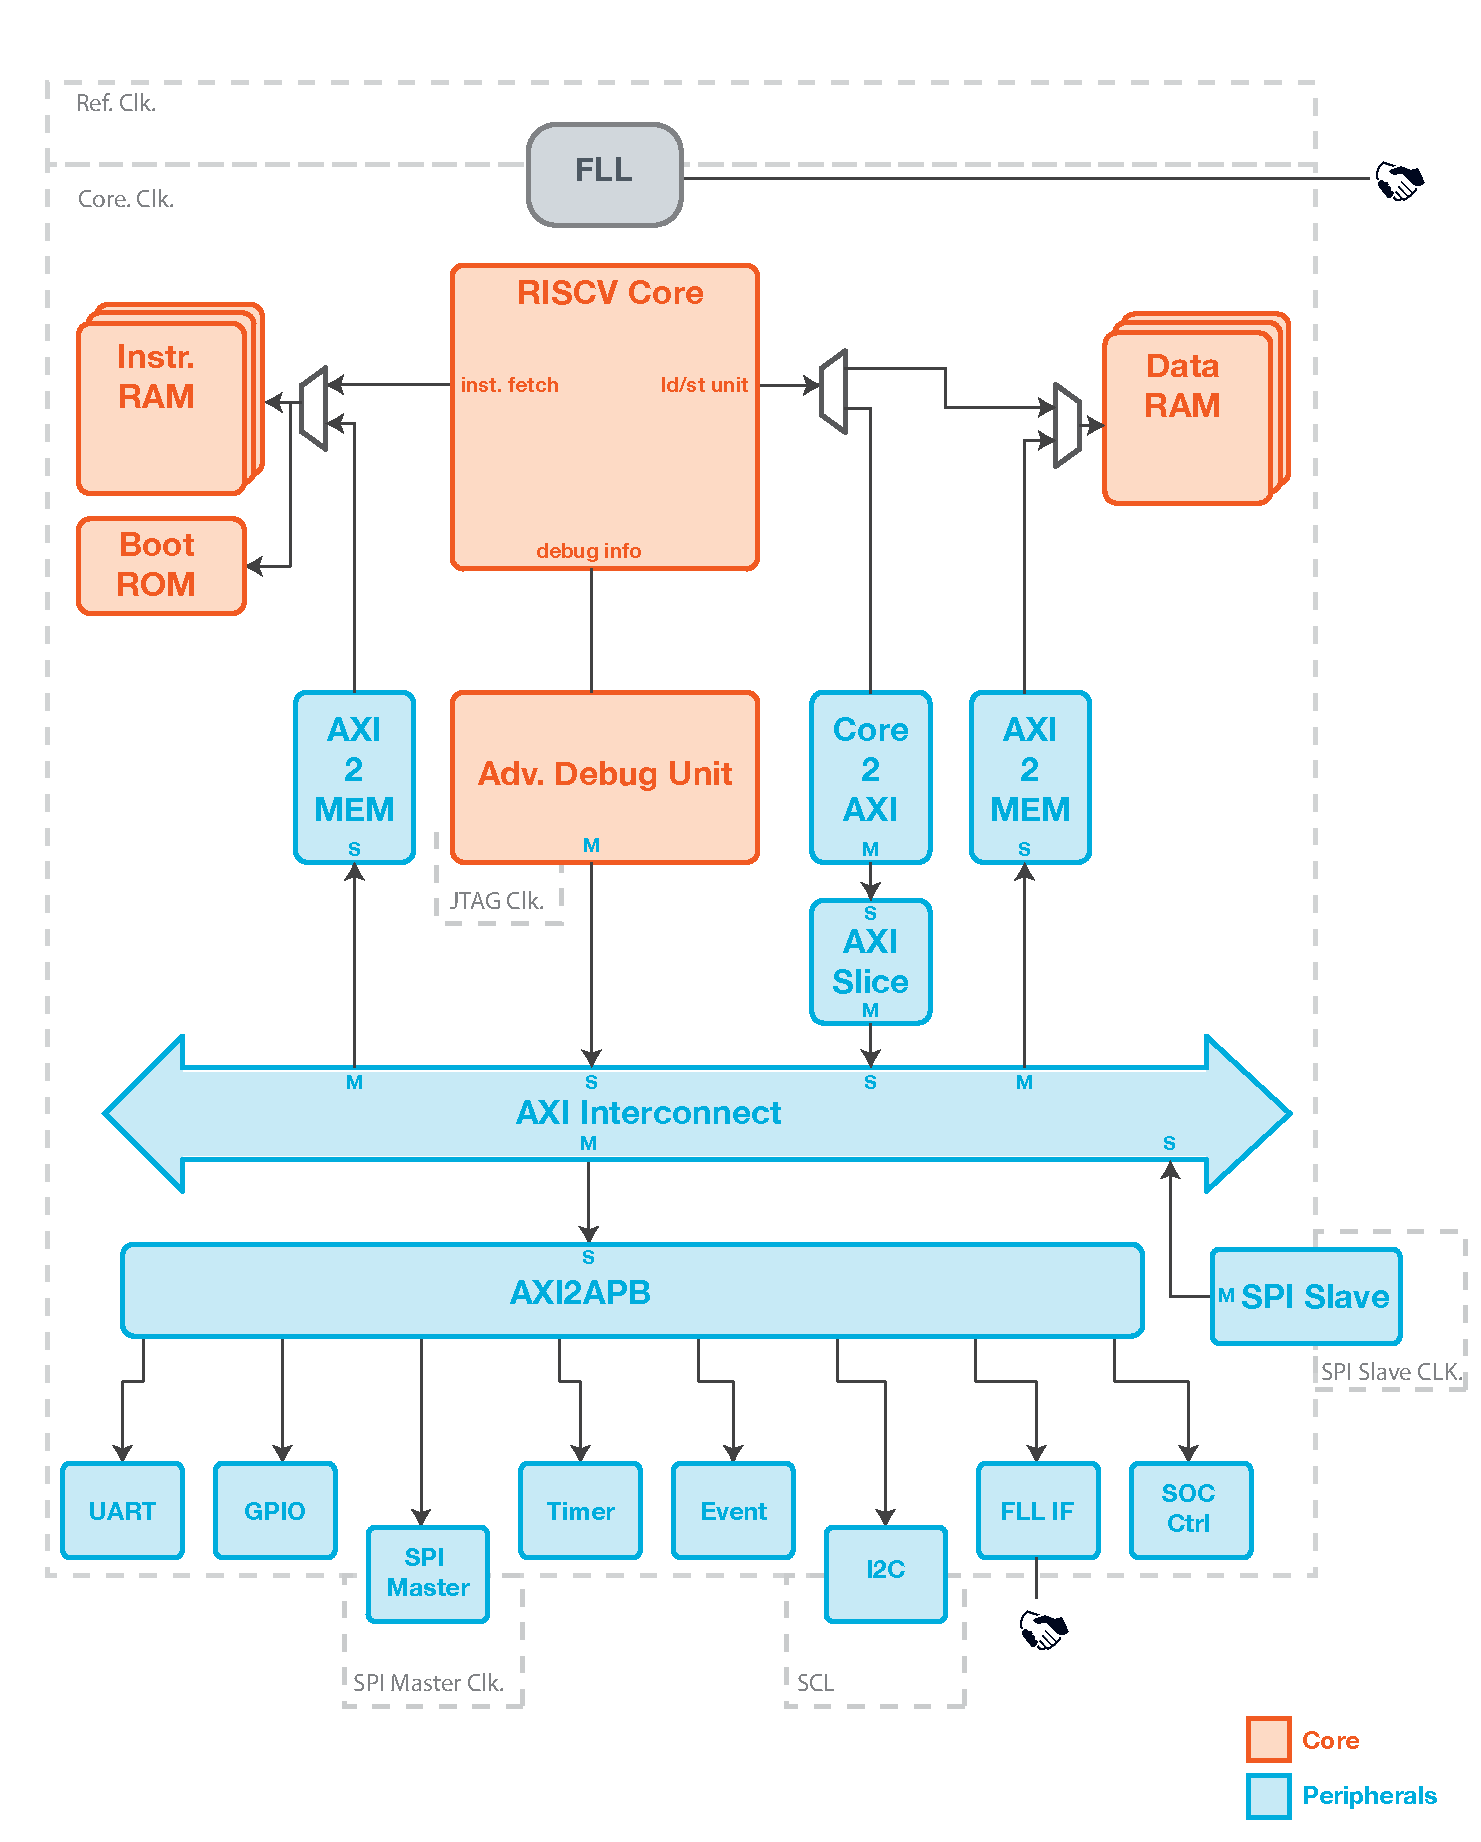
\includegraphics[width=\linewidth]{./figures/pulpino_blockdiagram}
  \caption{\pulpino block diagram}
  \label{fig:block_diagram}
\end{figure}


\section{Core}

\pulpino comes with two cores available. Both cores have been developed by the PULP group. This can either be the RISC-V core RI5CY or the pin compatible OpenRISC core OR10N.

\subsection{OpenRISC - OR10N}

OR10N was developed as part of a semester thesis here at IIS by Renzo Andri and Matthias Baer in 2014. It was meant to replace the former OpenRISC 1200 core used for the PULP project. The core employs a 32-bit 4 Stage in-order pipeline and has shown to be significantly faster then the reference implementation of the OpenCores community called OpenRISC 1200 \cite{renzobaer}.

\subsection{RISC-V - RI5CY}

RI5CY is a 4-stage in-order CPU based on the freely available RISC-V instruction set developed at UCB. The core has been mainly developed by Sven Stucki as part of his master's thesis (TODO: Citiation??). RI5CY is loosely based on OR10N. 

The RISC-V instruction set comes in a very modular and extendable flavor \cite{Waterman:EECS-2014-54}:

\begin{itemize}
    \item \textbf{RV32I}, \textbf{RV64I}: Is the 32-bit or 64-bit respectively, base integer instruction set. It describes general instruction formats and includes all operations to modify (integer) data and control flow. We fully support the bas integer instruction set with our RI5CY core.
    \item \textbf{M Standard Extension}: The M standard extension describes multiplication and division operations that multiply or divide values held in two integer registers. We provide only partial support for the M extension since our current multiplier implementation uses a single-cycle 32 bit lower result multiplier. As a matter of fact we do not support divisions and multiplications that return the upper half of the result.
    \item \textbf{A} (Atomic), \textbf{F} (single precision floating point) and \textbf{D} (double precision floating point) \textbf{standard extension}: We currently do not support any of these extensions.
    \item \textbf{C standard compressed ISA}: The compressed ISA specification is currently a proposal but will likely be frozen in the near future. The compressed ISA aims to reduce static and dynamic code size by adopting a simple compression scheme (i.e. small immediate values, one of the registers is the zero register $x0$,...). According to the current compressed ISA draft specification typically 50\%-60\% of the RISC-V instructions in a program can be replaced with RVC instructions, resulting in a 25\%-30\% code-size reduction~\cite{Waterman:EECS-2015-209}.
\end{itemize}

In addition the RISC-V ISA provides the opportunity to define instruction set extensions that are not currently officially supported. We do make particular use of this with support of post-increment load and store instructions, hardware loops and packed-SIMD instructions.


\section{AXI Interconnect}

\pulpino features an AXI bus as its main interconnect. Memories and the core are connected via dedicated bus adapters developed by the PULP group. The main advantage of having everything sharing one interconnect is the fact that the whole architecture becomes memory mapped. Resulting in the fact that 

% Axi slices

\subsection{SPI Slave}
\label{subsec:spi_slave}

\section{Advanced Debug Unit}

\section{APB Peripherals}

\subsection{Interrupt and Sleep Unit}

The unit is conducted as an APB peripheral. Each interrupt can be enabled or disabled and can have its pending status set or cleared by software (resulting in the fact that we support "soft interrupts"). The units main purpose is to keep track of all arriving interrupts and outputting the interrupt with the highest priority (starting from 0 up to 31) - iff it is enabled -  to the core in a one-hot encoded fashion. 

The interrupt unit can basically handle two types of interrupt sources:

\begin{itemize}
    \item \textbf{Pulsed interrupt request} - the interrupt request is at least one clock cycle long. When the interrupt controller receives a pulse at its interrupt input, the pending status is set and held until the interrupt gets served.
    \item L\textbf{evel triggered interrupt request} - the interrupt source holds the request high until the interrupt is serviced.
\end{itemize}

The interrupt output to the core is level sensitive. As long as there is a pending interrupt the corresponding interrupt request line (\verb+irq_o+) gets asserted. If the core wants to acknowledge an external interrupt it needs to clear the corresponding pending interrupt by writing 1 to the \verb+clear_pending+ (ICP) register. The interrupt is then de-asserted.

The event unit has exactly the same RTL layout as the interrupt unit. The only difference is that its \verb+signal_o+ is not forwarded to the processor core. An event can wake the core from sleep state. (TODO: provide a facility to get the currently pending event).

The sleep unit's task is to put the core into a low power mode by disabling its clock (through a clock gate). It therefore needs to track the sleep status of the core through a simple FSM (see figure~\ref{fig3}). The sleep unit is tightly coupled to the interrupt unit since it needs to wake the processor if an enabled interrupt arrives.
The sleep controller is as well conducted as an APB peripheral with two registers (see figure~\ref{fig4}):

\begin{enumerate}
    \item \textbf{Sleep Controll Register:} By writing the lowest bit (SE - Sleep Enable) to 1 the core requests to be put to sleep. Upon wakeup this bit is cleared by the controller.
    \item \textbf{Sleep Status Register:} This register contains the current sleep status of the core. This is helpful if for example you want to get the sleep status through the debug interface. Writes to this location are ignored.
\end{enumerate}

If the core signals that it is idle and wants to be put to sleep it writes the SE register. The controller then enters the \verb+SHUTDOWN+ state where the fetch enable signal of the core is de-asserted and no more instructions are fetched. After the processor has flushed its pipeline (signaled by a low \verb+core_busy+ signal) its clock is gated and the \verb+SLEEP+ state is entered. It now resides in a lower power state and can only be waked up by an external interrupt event (\verb+signal_i+ asserted).

\subsection{Timer Unit}

The timer provides a facility to cycle accurately time certain events and/or trigger interrupts or events respectively. In detail it should be possible to generate a timer overflow interrupt/event if the timer reaches its highest value and a timer output compare event when the timer is equal to a certain value set in the timer output compare register.


Additionally a timer control register makes it possible to set a pre-scaler, enable/disable timer overflow and timer output compare interrupts/events and to start and stop the timer respectively.

\subsection{\pulpino peripheral}
\label{subsec:pulpino_peripheral}

In order to control certain features of the SoC a special set of control registers is needed to do so. Since this is highly application specific (e.g. it only applies to this distinct SoC configuration) it has been my indention to logically and physically separate this sort of functionality into an independent peripheral.

Specificially this peripheral allows you to control the function of pads (e.g. whether they should be used as GPIO or perform there special function like SPI, UART, etc.). Furthermore this unit allows you to reconfigure the boot address. The boot address is the address the core stars fetching instructions as soon as the fetch enable signal of the core has been asserted.

\subsection{GPIO}
\label{subsec:gpio_peripheral}

\subsection{I2C}

\subsection{UART}

\subsection{SPI Master}








